\documentclass{ximera}
\title{Inverse Functions}

\outcome{Determine whether a function is one-to-one using the horizontal line test.}
\outcome{Verify that two functions are inverses using composition.}
\outcome{Find the inverse of a function algebraically.}
\outcome{State the domain and range of a function and its inverse.}
\outcome{Relate the graph of a function to the graph of its inverse.}

\begin{document}
\begin{abstract}
\end{abstract}
\maketitle

\textbf{Learning Objectives:}
\begin{itemize}
  \item Determine whether a function is one-to-one (horizontal line test).
  \item Verify inverse functions using composition: $(f\circ g)(x)=x$ AND $(g\circ f)(x)=x$.
  \item Find the inverse of a function algebraically; state its domain and range.
  \item Relate domain/range of $f$ to range/domain of $f^{-1}$; relate graphs via reflection over $y=x$.
\end{itemize}
\medskip

\noindent\textbf{One-to-One:} $f$ is one-to-one if $f(a)=f(b)\Rightarrow a=b$ (equivalently, its graph passes the horizontal line test).

\noindent\textbf{Inverse:} $g=f^{-1}$ if $(f\circ g)(x)=x$ \emph{and} $(g\circ f)(x)=x$.

\bigskip
\section*{Quick Check}

\begin{problem}
Let $f(x) = 3x-2$ and $g(x) = f^{-1}(x)$. What is the value of $f(g(5))$?
\begin{hint}
$f(f^{-1}(x)) = x$ by the definition of an inverse function.
\end{hint}
\begin{multipleChoice}
  \choice{$3$}
  \choice[correct]{$5$}
  \choice{$7$}
  \choice{$f$ and $g$ are not inverses}
  \choice{Cannot be determined}
\end{multipleChoice}
\end{problem}

\begin{problem}
Suppose a function $h$ has the values:
\begin{center}
\begin{tabular}{|c|c|c|c|c|}
\hline
$x$ & $-2$ & $0$ & $3$ & $5$ \\\hline
$h(x)$ & $4$ & $1$ & $7$ & $-3$ \\\hline
\end{tabular}
\end{center}
What is $h^{-1}(7)$?
\begin{hint}
$h^{-1}(7) = c$ means $h(c) = 7$. Find the input value that produces output 7.
\end{hint}
\begin{multipleChoice}
  \choice[correct]{$3$}
  \choice{$7$}
  \choice{$h(7)$ is undefined}
  \choice{$-3$}
  \choice{Not enough information}
\end{multipleChoice}
\end{problem}

\begin{problem}
The graph of $f$ is shown below (the line $f(x)=2x+1$ and the dashed line $y=x$).

\begin{center}
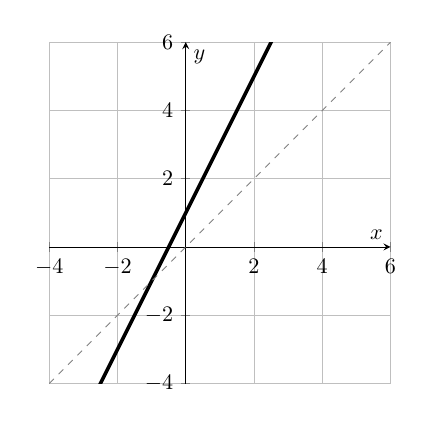
\begin{tikzpicture}[scale=0.8]
\begin{axis}[
  axis lines=middle,
  xmin=-4, xmax=6,
  ymin=-4, ymax=6,
  xtick={-4,-2,0,2,4,6},
  ytick={-4,-2,0,2,4,6},
  width=7cm, height=7cm,
  grid=both,
  xlabel={$x$}, ylabel={$y$}
]
\addplot[ultra thick, black, domain=-3:4] {2*x + 1};
\addplot[dashed, gray, domain=-4:6] {x};
\end{axis}
\end{tikzpicture}
\end{center}

Which of the following best describes the graph of $f^{-1}$?
\begin{hint}
Solve $y=2x+1$ for $x$ to get $f^{-1}$. The graph of $f^{-1}$ is the reflection of $f$ across the line $y=x$.
\end{hint}
\begin{multipleChoice}
  \choice[correct]{A line with slope $\dfrac{1}{2}$ passing through $(1,0)$}
  \choice{A line with slope $2$ passing through $(0,1)$}
  \choice{A line reflected across $y=-x$}
  \choice{Not a function}
  \choice{A parabola opening up}
\end{multipleChoice}
\end{problem}

\begin{problem}
Let $f(x) = \sqrt{x+4}$ and $g(x) = x^2-4$. Which of the following is true?
\begin{hint}
Compute $g(f(x)) = (\sqrt{x+4})^2-4 = x$, valid for $x \geq -4$ (the domain of $f$). Then check whether $f(g(x)) = |x| = x$ only for $x \geq 0$, not on the full domain of $g$.
\end{hint}
\begin{multipleChoice}
  \choice{$f$ and $g$ are inverses on their entire domains}
  \choice{$f(g(x)) = x$ for all $x \geq 2$}
  \choice[correct]{$g(f(x)) = x$ for all $x \geq -4$}
  \choice{$f(g(x))$ is undefined for $x=0$}
  \choice{$f$ and $g$ have the same domain}
\end{multipleChoice}
\end{problem}

\begin{problem}
A temperature sensor outputs voltage $V$ related to temperature $T$ by $V = 0.5T + 1.2$. What is the formula for the inverse function $T(V)$?
\begin{hint}
Solve for $T$: subtract 1.2, then divide by 0.5. Note that $\dfrac{V-1.2}{0.5}$ and $2(V-1.2)$ are equivalent.
\end{hint}
\begin{multipleChoice}
  \choice[correct]{$T(V) = \dfrac{V-1.2}{0.5}$}
  \choice{$T(V) = 2V+1.2$}
  \choice{$T(V) = 0.5V-1.2$}
  \choice{$T(V) = 2(V-1.2)$}
  \choice{$T(V) = \dfrac{V+1.2}{0.5}$}
\end{multipleChoice}
\end{problem}


\bigskip
\section*{Extended Practice}

\begin{problem}
Determine whether each function is one-to-one. If not, suggest a domain restriction that makes it one-to-one.
\begin{enumerate}
  \item[(a)] $f(x) = x^2+2$
  \item[(b)] $g(x) = x^3-8$
  \item[(c)] $q(x) = |x-3|$
  \item[(d)] $h(x) = 4x^4-4x^3+1$
  \item[(e)] $d(x) = \sqrt[3]{1-4x}$
  \item[(f)] $b(x) = \sqrt{2x+3}$
\end{enumerate}

\begin{solution}
\begin{enumerate}
  \item[(a)] \textbf{Not one-to-one.} $f(1)=f(-1)=3$. Restrict to $(-\infty,0]$ or $[0,\infty)$.
  \item[(b)] \textbf{Yes.} $y=x^3-8$ gives $x=\sqrt[3]{y+8}$, a unique $x$ for each $y$.
  \item[(c)] \textbf{Not one-to-one.} $q(0)=q(6)=3$. Restrict to $(-\infty,3]$ or $[3,\infty)$.
  \item[(d)] \textbf{Not one-to-one.} As an even-degree polynomial, $h(x)\to+\infty$ as $x\to\pm\infty$, so it fails the horizontal line test.
  \item[(e)] \textbf{Yes.} $y=\sqrt[3]{1-4x}$ gives $x=\tfrac{1}{4}(1-y^3)$, unique for each $y$.
  \item[(f)] \textbf{Yes.} The square root function is increasing on its domain, so it is one-to-one.
\end{enumerate}
\end{solution}
\end{problem}


\begin{problem}
Show that each pair of functions are inverses of each other using composition.
\begin{enumerate}
  \item[(a)] $h(x) = 7x-3$;\quad $k(x) = \dfrac{x+3}{7}$
  \medskip
  \item[(b)] $m(x) = 10-(3+5x)^3$;\quad $n(x) = \dfrac{\sqrt[3]{10-x}-3}{5}$
  \medskip
  \item[(c)] $f(x) = \dfrac{2x+1}{x+4}$;\quad $g(x) = \dfrac{1-4x}{x-2}$
\end{enumerate}

\begin{solution}
\begin{enumerate}
  \item[(a)]
  \begin{align*}
    h(k(x)) &= 7\!\cdot\!\frac{x+3}{7}-3 = x+3-3 = x \quad\checkmark\\
    k(h(x)) &= \frac{(7x-3)+3}{7} = \frac{7x}{7} = x \quad\checkmark
  \end{align*}

  \item[(b)]
  \begin{align*}
    m(n(x)) &= 10-\!\left[3+5\cdot\frac{\sqrt[3]{10-x}-3}{5}\right]^3 = 10-\!\left[\sqrt[3]{10-x}\right]^3 = 10-(10-x) = x \quad\checkmark\\
    n(m(x)) &= \frac{\sqrt[3]{10-(10-(3+5x)^3)}-3}{5} = \frac{\sqrt[3]{(3+5x)^3}-3}{5} = \frac{(3+5x)-3}{5} = x \quad\checkmark
  \end{align*}

  \item[(c)] Multiply top and bottom by $(x-2)$ (or $(x+4)$) to clear fractions:
  \begin{align*}
    f(g(x)) &= \frac{2\!\cdot\!\frac{1-4x}{x-2}+1}{\frac{1-4x}{x-2}+4} = \frac{2(1-4x)+(x-2)}{(1-4x)+4(x-2)} = \frac{-7x}{-7} = x \quad\checkmark\\
    g(f(x)) &= \frac{1-4\!\cdot\!\frac{2x+1}{x+4}}{\frac{2x+1}{x+4}-2} = \frac{(x+4)-4(2x+1)}{(2x+1)-2(x+4)} = \frac{-7x}{-7} = x \quad\checkmark
  \end{align*}
\end{enumerate}
\end{solution}
\end{problem}


\begin{problem}
For each function: find (i) domain and range of $f$, (ii) $f^{-1}(x)$, (iii) domain and range of $f^{-1}$.
\begin{enumerate}
  \item[(a)] $f(x) = \dfrac{4-x}{9}$
  \medskip
  \item[(b)] $m(x) = 4x^3+2$
  \medskip
  \item[(c)] $s(x) = \dfrac{2}{x-3}$
  \medskip
  \item[(d)] $v(x) = \dfrac{2x-1}{x-2}$
  \medskip
  \item[(e)] $f(x) = x^2+1,\quad x\leq 0$
  \medskip
  \item[(f)] $g(x) = \sqrt{2x-4}$
\end{enumerate}

\begin{solution}
\begin{enumerate}
  \item[(a)] Domain: $(-\infty,\infty)$; Range: $(-\infty,\infty)$.
  Swap and solve: $x=\tfrac{4-y}{9}\Rightarrow y=4-9x$. So $f^{-1}(x)=4-9x$.
  Domain of $f^{-1}$: $(-\infty,\infty)$; Range of $f^{-1}$: $(-\infty,\infty)$.

  \item[(b)] Domain: $(-\infty,\infty)$; Range: $(-\infty,\infty)$.
  $y=4x^3+2\Rightarrow x=\sqrt[3]{\tfrac{y-2}{4}}$. So $m^{-1}(x)=\sqrt[3]{\dfrac{x-2}{4}}$.
  Domain of $m^{-1}$: $(-\infty,\infty)$; Range: $(-\infty,\infty)$.

  \item[(c)] Domain: $(-\infty,3)\cup(3,\infty)$; Range: $(-\infty,0)\cup(0,\infty)$.
  $y=\tfrac{2}{x-3}\Rightarrow x-3=\tfrac{2}{y}\Rightarrow x=\tfrac{2}{y}+3$. So $s^{-1}(x)=\dfrac{2+3x}{x}$.
  Domain of $s^{-1}$: $(-\infty,0)\cup(0,\infty)$; Range: $(-\infty,3)\cup(3,\infty)$.

  \item[(d)] Domain: $(-\infty,2)\cup(2,\infty)$; Range: $(-\infty,2)\cup(2,\infty)$.
  $y=\tfrac{2x-1}{x-2}\Rightarrow y(x-2)=2x-1\Rightarrow yx-2x=2y-1\cdot\Rightarrow x(y-2)=2y-1\Rightarrow x=\tfrac{2y-1}{y-2}$.
  So $v^{-1}(x)=\dfrac{2x-1}{x-2}=v(x)$ (the function is its own inverse).
  Domain of $v^{-1}$: $(-\infty,2)\cup(2,\infty)$; Range: $(-\infty,2)\cup(2,\infty)$.

  \item[(e)] Domain: $(-\infty,0]$; Range: $[1,\infty)$.
  $y=x^2+1\Rightarrow x^2=y-1\Rightarrow x=\pm\sqrt{y-1}$. Since $x\leq0$, take $x=-\sqrt{y-1}$.
  $f^{-1}(x)=-\sqrt{x-1}$.
  Domain of $f^{-1}$: $[1,\infty)$; Range: $(-\infty,0]$.

  \item[(f)] Domain: $[2,\infty)$; Range: $[0,\infty)$.
  $y=\sqrt{2x-4}\Rightarrow x=\sqrt{2y-4}\Rightarrow x^2=2y-4\Rightarrow y=\tfrac{x^2+4}{2}$.
  $g^{-1}(x)=\dfrac{1}{2}x^2+2$, with $x\geq0$.
  Domain of $g^{-1}$: $[0,\infty)$; Range: $[2,\infty)$.
\end{enumerate}
\end{solution}
\end{problem}


\begin{problem}
The graph of $h(x)$ has domain $[-5,3]$ (see handout). The graph passes through points including $(-5,-3)$, $(0,3)$, and $(3,4)$ (approximate).

\begin{enumerate}
  \item[(a)] Describe how to sketch $h^{-1}(x)$ and identify corresponding points.
  \item[(b)] Find the domain and range of $h^{-1}(x)$.
\end{enumerate}

\begin{solution}
\begin{enumerate}
  \item[(a)] Reflect the graph of $h$ over the line $y=x$: every point $(x,y)$ on $h$ maps to $(y,x)$ on $h^{-1}$. For example, $(0,3)$ on $h$ gives $(3,0)$ on $h^{-1}$.

  \item[(b)] The domain of $h^{-1}$ equals the range of $h$: $[-3,4]$.\\
  The range of $h^{-1}$ equals the domain of $h$: $[-5,3]$.
\end{enumerate}
\end{solution}
\end{problem}

\end{document}
